\chapter{Esercizio a scelta}
\section{Traccia}

 Modifica di esercizi già proposti (processore, rete di interconnessione o interfaccia seriale) mediante aggiunta/aggiornamento di funzionalità. 
Esempio: si potrebbe pensare di modificare l’interfaccia seriale aggiungendo segnali specifici per l’\textit{handshaking} fra due entità. 

\subsection{Descrizione esercizio}
Partendo da gli esercizi numero 7 e 9 si è scelto di creare un unico sistema che comprende le funzionalità di trasmissione seriale ripetuta, tracciata da un contatore, la sincronizzazione tramite three-way handshake e la lettura e scrittura su memoria con l'esecuzione di un'operazione di somma.


\subsection{Architettura}
L'architettura unisce diversi aspetti degli esercizi precedenti. Ci sono due componenti, A e B che comunicano tramite un'interfaccia seriale UART. Le due unità di controllo in A e B sono connesse con tre segnali per effettuare il three-way handshake necessario alla sincronizzazione della trasmissione.

Il sistema A è composto da:
\begin{itemize}
    \item \textit{ROM}: è una memoria che contiene le N stringe di 8 bit da dover mandare al sistema B;
    \item \textit{UART}: il componente, fornitoci a priori, costituisce in un'interfaccia per la trasmissione del dato tra i due sistemi;
    \item \textit{contatore}: conta il numero di trasmissioni effettuate;
    \item \textit{rete di controllo}: regola che la trasmissione dei dati avvenga in modo corretto.
\end{itemize}

Il sistema B, invece, è composto da:
\begin{itemize}
    \item \textit{registro}: un flip flop che memorizza la stringa ricevuta dal sistema A;
    \item \textit{UART}: il componente, fornitoci a priori, costituisce in un'interfaccia per la ricezione del dato ;
    \item \textit{contatore}: conta il numero di trasmissioni effettuate, nonché il numero di somme effettuate;
    \item \textit{ROM}: è una memoria che contiene le N stringe da sommare;
    \item \textit{rete di controllo}: regola che la trasmissione e l'output dei dati avvenga in modo corretto.
\end{itemize}

L'interconnessione tra i due sistemi è visibile nella seguente architettura: 
\begin{figure}[H]
    \centering
    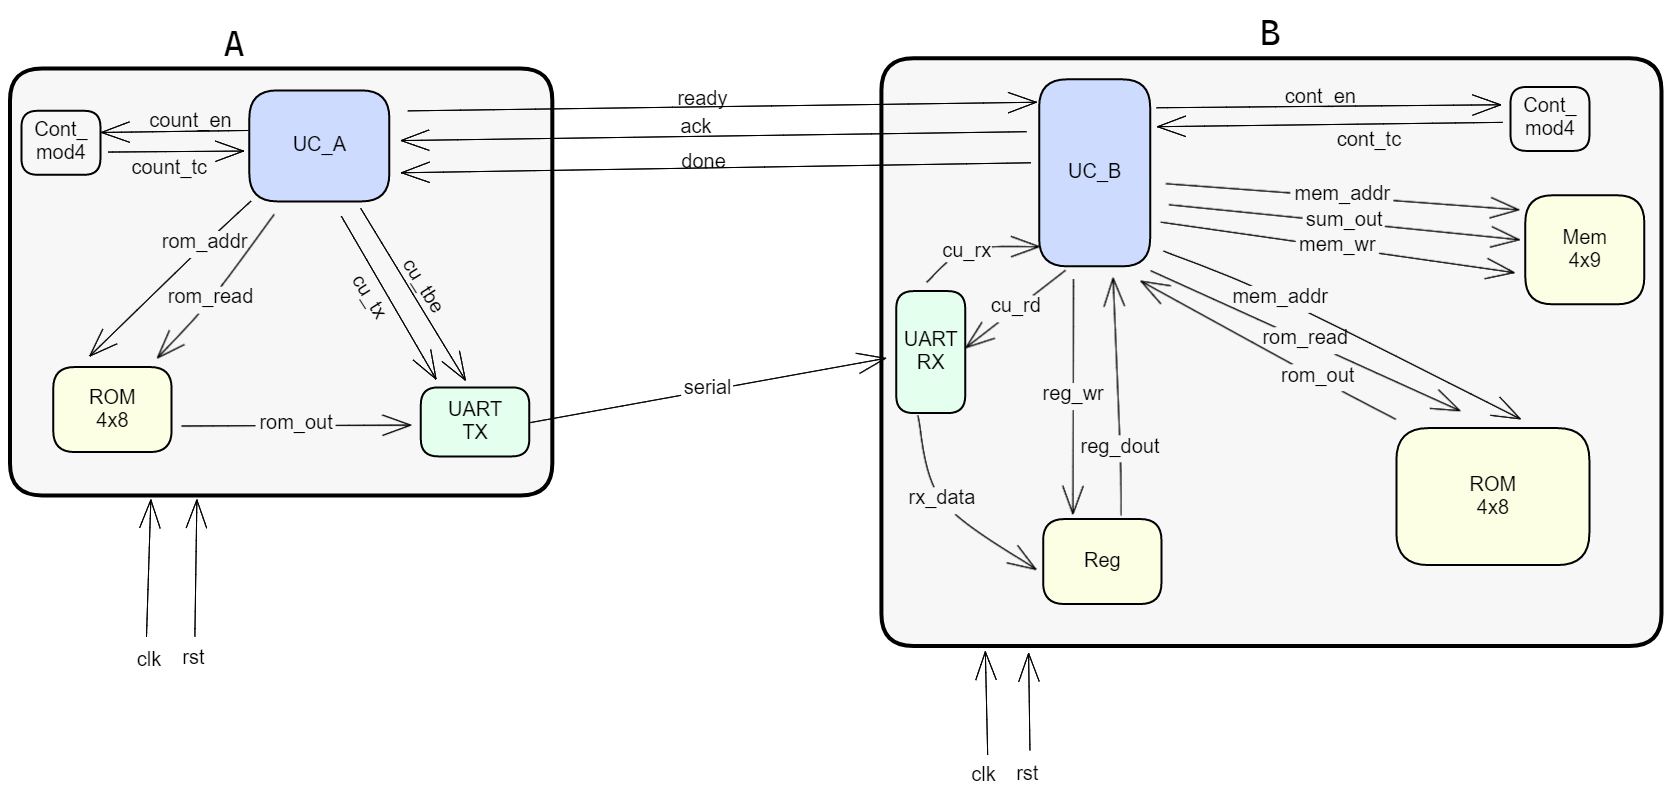
\includegraphics[width=16cm]{immagini/esercizio12/schema_12.png}
    \caption{Schema Interfaccia Seriale}
\end{figure}

Gli automi di A e B sono basati su quelli visti nei precedenti esercizi ma hanno subito diverse modifiche.
Nel sistema A prima di poter abilitare il segnale di \textit{ready} viene effettuata la lettura dalla memoria ROM in cui sono contenuti i dati da trasmettere. Successivamente si aspetta l'ack del sistema B, che indica la sua disponibilità a ricevere il dato. Questo punto è essenziale, poichè significa che B ha impostato il ricevitore UART in modo opportuno. Superato l'ack l'automa controlla che il segnale tbe sia uguale a 1. In caso contrario, significa che il trasmettitore è occupato, e non può ancora inviare messaggi. Appena il trasmettitore è pronto, viene alzato cu\_tx e si aspetta la fine della ricezione del dato da parte di B, indicata dal segnale \textit{done}.\\

È da notare che allo stato successivo è stato inserito un altro auto-anello che aspetta che il \textit{done} si abbassi. Questo stato serve per evitare che il cambiamento del segnale \textit{done} risvegli il processo durante uno stato sensibile, come ad esempio quello in cui si incrementa l'indirizzo (si avrebbe un incremento doppio). Non è possibile per A controllare quando il segnale \textit{done} varierà, e questa misura quindi si aggiunge alle regole del protocollo stabilito che mira ad incrementare l'affidabilità della trasmissione. \\

Si sarebbero potute implementare soluzioni alternative, come l'utilizzo di clock più lenti o l'aggiunta di stati, ma questa soluzione con il ciclo permette all'automa di funzionare a prescindere dalla tecnologia sottostante, senza andare a inficiare sui tempi del clock.

Infine, viene incrementato il contatore e l'indirizzo di memoria, e si esegue il controllo sul \textit{count\_tc}. Una volta alzato infatti, l'automa arriverà allo stato \textit{idle} e fermerà le trasmissioni.


L'automa di B aspetta e alza i segnali ready e ack in modo duale ad A , e una volta arrivato il messaggio, notificato dal segnale alto \textit{RDA (uc\_rx)} scrive il risultato in un registro temporaneo. A questo punto l'interfaccia UART è libera, e si procede alla lettura della ROM di B e alla somma con il dato appena arrivato. Finita la somma, a cui è stato dato il tempo di finire con uno stato a se, il risultato viene scritto in una memoria e si controlla se si è arrivati al massimo delle ricezioni possibili. 

Di seguito è possibile osservare la stesura degli automi dei singoli sistemi: 
\begin{figure}[H]
    \centering
    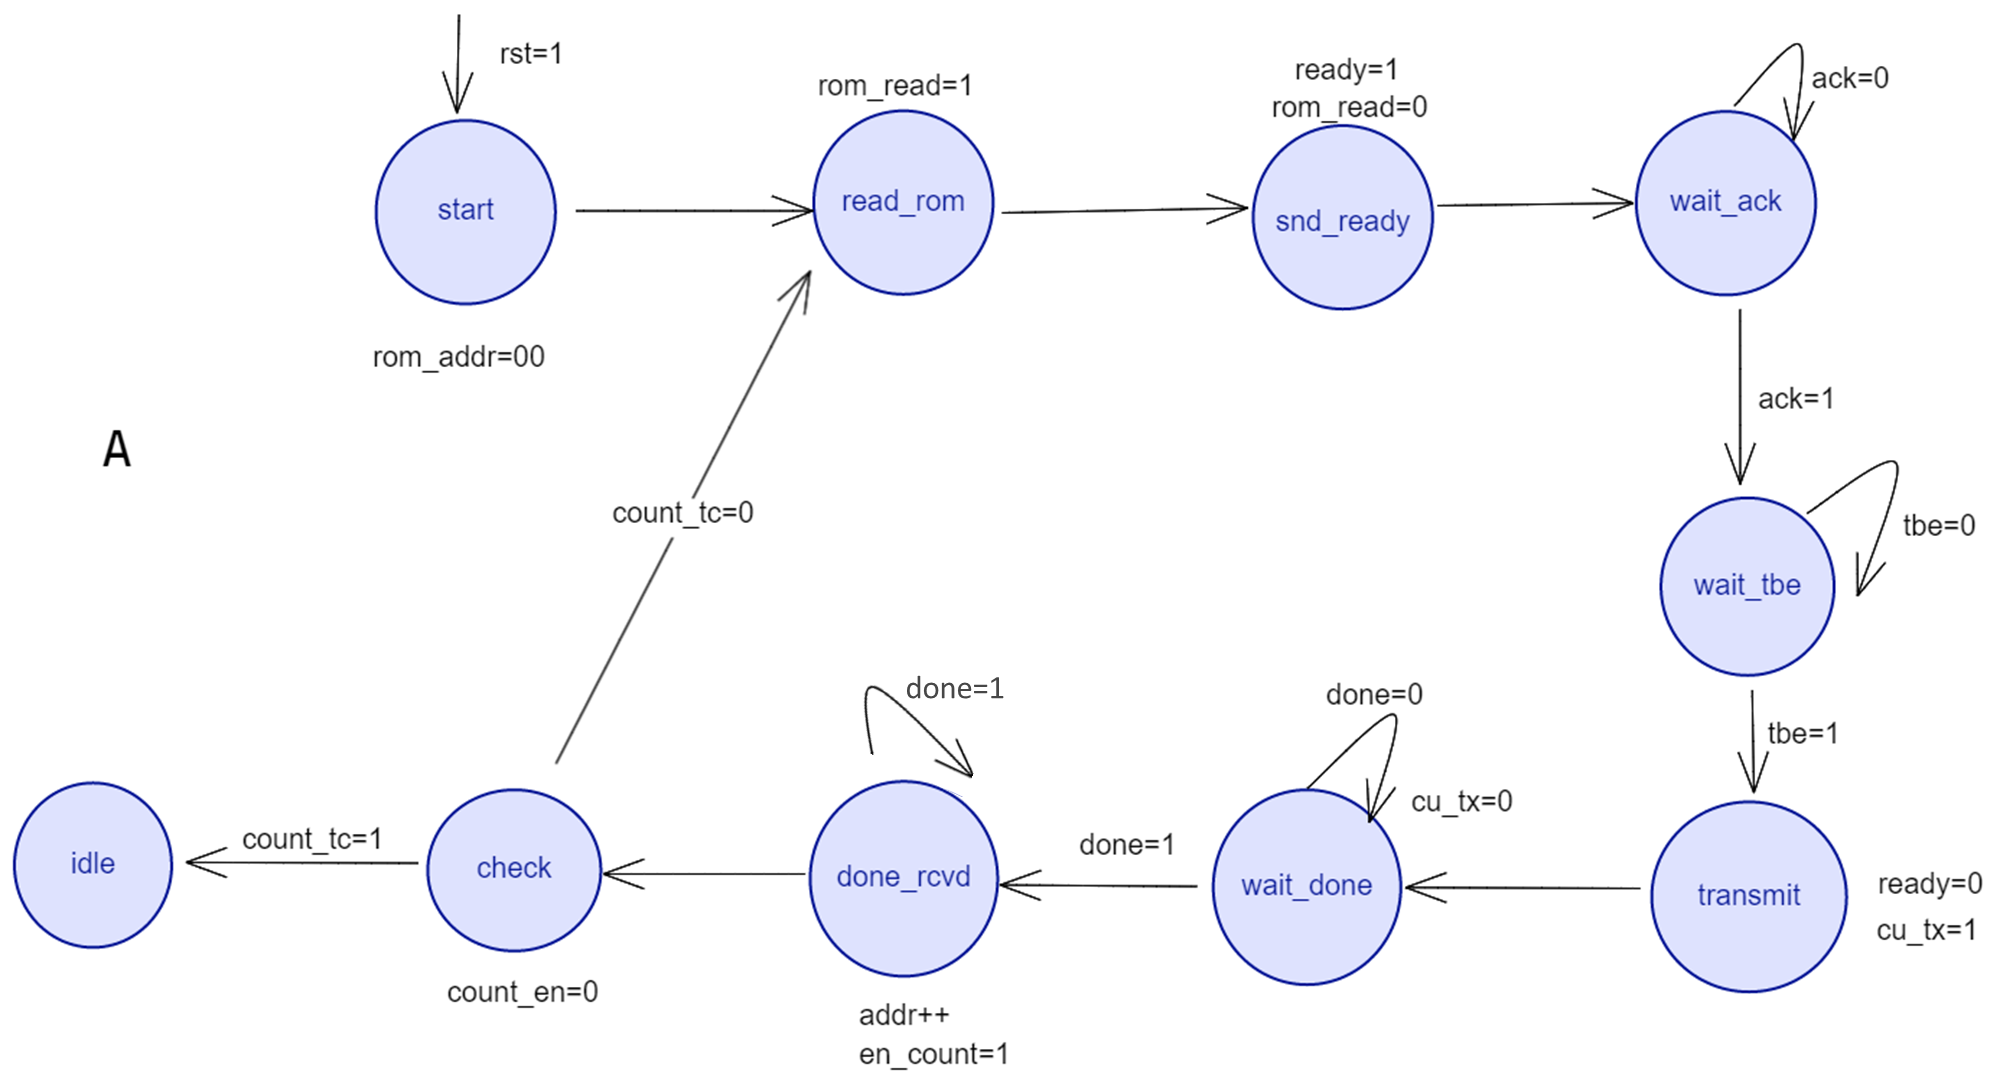
\includegraphics[width=16cm]{immagini/esercizio12/automaA_12.png}
    \caption{Automa A}
\end{figure}

\begin{figure}[H]
    \centering
    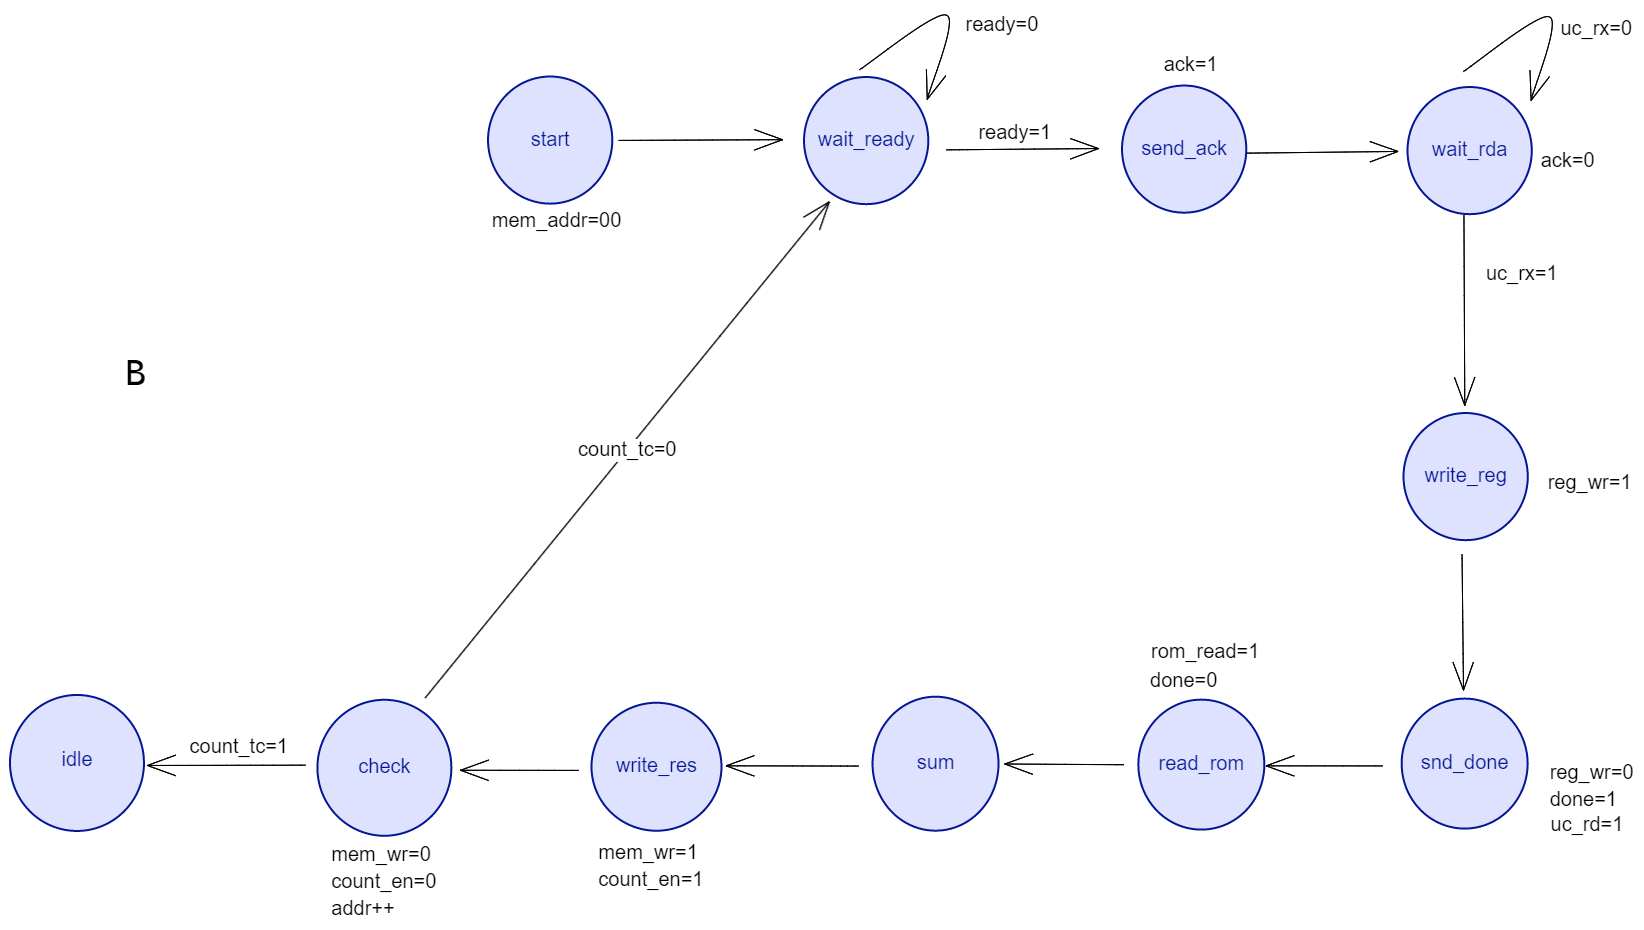
\includegraphics[width=16cm]{immagini/esercizio12/automaB_12.png}
    \caption{Automa B}
\end{figure}

\subsection{Analisi}
\subsubsection{UART vs USART}
L'idea della soluzione si basa sul confronto tra UART e USART e le performance nettamente superiori della versione sincrona rispetto a quella asincrona. In particolare, in Tabella \ref{tab:uart_usart}, sono analizzate le differenze tra le due tecnologie.

\begin{table}
    \centering
    \begin{tabular}{|p{5cm}||p{5cm}| }
        \hline
        UART & USART \\ [0.5ex] 
         \hline\hline
         \hline
            Può comunicare sia in \textit{half-duplex} che \textit{full-duplex} & Può comunicare \textbf{solo} in modalità \textit{half-duplex} \\
         \hline 
         \hline
           Invia dati con \textit{rate} diversi, di solito più basso rispetto all'USART & Invia dati con un rate fisso  \\
         \hline
            Sorgente e destinazione devono essere configurati con i parametri corretti del \textit{baud rate} & Sorgente e destinazione non hanno bisogno di conoscere nulla dei rispettivi \textit{clock} \\
         \hline
         Invia un byte per volta & Può inviare pacchetti più grandi \\
         \hline
          
    \end{tabular}
    \caption{Confronto tra UART e USART}
    \label{tab:uart_usart}
\end{table}


Uno dei motivi per cui è molto diffuso UART è per la sua facilità di implementazione. Con l'approccio scelto si preserva la semplicità, ma si aggiunge un grado di affidabilità alla comunicazione. Inoltre, utilizzando la periferica UART è possibile continuare ad effettuare comunicazioni \textit{full-duplex}.



\subsubsection{Three-way-handshake vs Two-way-handshake}

Nell'esercizio svolto, sono combinati i benefici sia del mondo sincrono che quello asincrono. Infatti, la soluzione prevede di implementare l'handshake e quindi la gestione della sincronizzazione tra le due entità al di fuori della periferica UART. In questo modo, la comunicazione risulta sincrona (anche se i due sistemi devono conoscere il \textit{baud rate}), e in caso di errori di trasmissione, il ricevitore può usare il segnale \textit{done} per codificare una politica di gestione del \textit{fault}. Ad esempio, immaginando di avere più bit per il segnale \textit{done}, può essere codificato un codice di risposta in cui si richiede una ritrasmissione.


Di seguito è riportato il codice dell'intera soluzione, omettendo i componenti elementari quali flip flop e memoria già descritti nei capitoli precedenti.
\begin{lstlisting} [language=VHDL, caption=Rete di controllo di A]
library IEEE;
use IEEE.STD_LOGIC_1164.ALL;
use IEEE.numeric_std.all;

entity cu_a is
    port(
        clk, rst, ack, done, count_tc, cu_tbe: in std_logic;
        ready, cu_tx, rom_read, count_en: out std_logic;
        rom_addr: out std_logic_vector(1 downto 0)
    );
end cu_a;

architecture behavioral of cu_a is

    type state is (
        START,
        READ_ROM,
        SND_READY,
        WAIT_ACK,
        WAIT_TBE,
        TRANSMIT,
        WAIT_DONE,
        INCR_ADDR,
        DONE_RCVD,
        CHECK,
        IDLE
    );
    signal current_state : state:= IDLE;
    signal next_state : state;
    signal s_addr: std_logic_vector(1 downto 0) := "00";

begin
    comb: process(current_state, ack, done, cu_tbe)
    begin
        case current_state is

            when START =>
                ready <= '0';
                s_addr <= "00";
                rom_read <= '0';
                cu_tx <= '0';
                count_en <= '0';
                next_state<= READ_ROM;

            when READ_ROM=>
                rom_read <= '1';
                next_state <= SND_READY;

            when SND_READY=>
                rom_read <= '0';
                ready <= '1';
                next_state <= WAIT_ACK;

            when WAIT_ACK=>
                if ( ack = '1' ) then
                    next_state <= WAIT_TBE;
                else
                    next_state <= WAIT_ACK;
                end if;

            when WAIT_TBE =>
                if cu_tbe = '1' then
                    next_state <= TRANSMIT;
                else
                    next_state <= WAIT_TBE;
                end if;

            when TRANSMIT=>
                cu_tx <= '1';
                ready <= '0';
                next_state <= WAIT_DONE;

            when WAIT_DONE=>
                cu_tx <= '0';
                if ( done = '1' ) then
                    next_state <= DONE_RCVD;
                else
                    next_state <= WAIT_DONE;
                end if;

            when DONE_RCVD=>
                count_en <= '1';
                if done = '0' then
                    next_state <= INCR_ADDR;
                else 
                    next_state <= DONE_RCVD;
                end if;

           when INCR_ADDR =>
                s_addr <= std_logic_vector((unsigned(s_addr) + 1));
                next_state <= CHECK;
    
            when CHECK =>
                count_en <= '0';
                if count_tc = '1' then
                    next_state <= IDLE;
                else
                    next_state <= READ_ROM;
                end if;

            when IDLE=>
                next_state<= IDLE;
            when others => next_state<= IDLE;
        end case;
    end process comb;

    rom_addr <= s_addr;

    seq: process(clk)
    begin
        if rising_edge(clk) then
            if rst='1'  then
                current_state<=START;
            else
                current_state<=next_state;
            end if;
        end if;
    end process seq;
end behavioral;
\end{lstlisting}

\begin{lstlisting} [language=VHDL, caption=Rom di A]
library ieee;
use ieee.std_logic_1164.all;
use ieee.numeric_std.all;

entity rom_a is
port(
    clk, read : in std_logic; 
    addr : in std_logic_vector(1 downto 0);
    data : out std_logic_vector(7 downto 0)
    );
end rom_a;

architecture behavioral of rom_a is 
type rom_t is array (0 to 3) of std_logic_vector(7 downto 0);
signal rom : rom_t := (
    "00000010", 
    "00000110", 
    "00001001", 
    "00001111"
);

begin

process(clk)
  begin
    if rising_edge(clk) then
        if read = '1' then
            data <= rom(to_integer(unsigned(addr)));
        end if;
    end if;
end process;
end behavioral;
\end{lstlisting}

Di seguito il codice di A:
\begin{lstlisting} [language=VHDL, caption=Sistema A]
library IEEE;
use IEEE.STD_LOGIC_1164.ALL;

entity a is
    Port (
        clk, ack, rst, done: in std_logic ;
        ready, data: out std_logic
    );
end a;

architecture Structural of a is

    component cont_mod4 is
        port (
            clk, rst: in std_logic;
            tc: out std_logic
        );
    end component cont_mod4;

    component cu_a is
        port(
            clk, rst, ack, done, count_tc, cu_tbe: in std_logic;
            ready, cu_tx, rom_read, count_en : out std_logic;
            rom_addr: out std_logic_vector(1 downto 0)
        );
    end component cu_a;

    component rom_a is
        port(
            clk, read : in std_logic;
            addr : in std_logic_vector(1 downto 0);
            data : out std_logic_vector(7 downto 0)
        );
    end component rom_a;

    component UARTcomponent is
        Generic (
            --@48MHz
            --		BAUD_DIVIDE_G : integer := 26; 	--115200 baud
            --		BAUD_RATE_G   : integer := 417

            --@26.6MHz
            BAUD_DIVIDE_G : integer := 14; 	--115200 baud
            BAUD_RATE_G   : integer := 231
        );
        Port (
            TXD 	: out 	std_logic  	:= '1';					-- Transmitted serial data output
            RXD 	: in  	std_logic;							-- Received serial data input
            CLK 	: in  	std_logic;							-- Clock signal
            DBIN 	: in  	std_logic_vector (7 downto 0);		-- Input parallel data to be transmitted
            DBOUT 	: out 	std_logic_vector (7 downto 0);		-- Recevived parallel data output
            RDA		: inout  std_logic;							-- Read Data Available
            TBE		: out 	std_logic 	:= '1';					-- Transfer Buffer Emty
            RD		: in  	std_logic;							-- Read Strobe
            WR		: in  	std_logic;							-- Write Strobe
            PE		: out 	std_logic;							-- Parity error		
            FE		: out 	std_logic;							-- Frame error
            OE		: out 	std_logic;							-- Overwrite error
            RST		: in  	std_logic	:= '0');				-- Reset signal
    end component  UARTcomponent;

    signal count_en, count_tc, rom_read, cu_tx, cu_tbe: std_logic := '0';
    signal rom_addr: std_logic_vector(1 downto 0) := "00";
    signal rom_out: std_logic_vector(7 downto 0) := "00000000";

begin

    cont : cont_mod4
        port map(
            clk=>count_en,
            rst=>rst,
            tc=>count_tc
        );

    cu : cu_a
        port map(
            clk=>clk,
            rst=>rst,
            count_tc=>count_tc ,
            count_en => count_en,
            rom_addr=>rom_addr,
            rom_read=>rom_read,
            ready=>ready,
            done => done,
            ack=>ack,
            cu_tx => cu_tx,
            cu_tbe=>cu_tbe
        );

    rom : rom_a
        port map(
            clk=>clk,
            read=>rom_read,
            addr=>rom_addr,
            data=>rom_out
        );

    uart:  UARTcomponent generic map(
            BAUD_DIVIDE_G=>26,
            BAUD_RATE_G=>417
        )
        port map (
            TXD => data,
            RXD => '1',
            CLK => clk,
            DBIN => rom_out,
            DBOUT => OPEN,
            RDA => OPEN,
            TBE => cu_tbe,
            RD => '0',
            WR => cu_tx,
            PE => OPEN,
            FE => OPEN,
            OE => OPEN,
            RST => rst
        );

end Structural;
\end{lstlisting}

N.B.: il codice del contatore mod4 coincide con il codice del contatore del sistema A e per semplicità è stato omesso il codice della UART.

\begin{lstlisting} [language=VHDL, caption=Rom di B]
library ieee;
use ieee.std_logic_1164.all;
use ieee.numeric_std.all;

entity rom_b is
port(
    clk, read : in std_logic; 
    addr : in std_logic_vector(1 downto 0);
    data : out std_logic_vector(7 downto 0)
    );
end rom_b;

architecture behavioral of rom_b is 
type rom_t is array (0 to 3) of std_logic_vector(7 downto 0);
signal rom : rom_t := (
    "00000001", 
    "00000001", 
    "00000001", 
    "00000001"
);

begin

process(clk)
  begin
    if rising_edge(clk) then
        if read = '1' then
            data <= rom(to_integer(unsigned(addr)));
        end if;
    end if;
end process;
end behavioral;
\end{lstlisting}


\begin{lstlisting} [language=VHDL, caption=Rete di controllo di B]
library IEEE;
use IEEE.STD_LOGIC_1164.ALL;
use IEEE.numeric_std.all;

entity cu_b is
    port(
        clk, rst, ready,  count_tc, cu_rx: in std_logic;
        rom_out, reg_dout : in std_logic_vector(8 downto 0);
        ack, done, count_en, rom_read, reg_wr, mem_wr, cu_rd: out std_logic;
        mem_addr: out std_logic_vector(1 downto 0);
        sum_out: out std_logic_vector(8 downto 0)
    );
end cu_b;

architecture behavioral of cu_b is

    type state is (
        START,
        WAIT_READY,
        SEND_ACK,
        WAIT_RDA,
        WRITE_REG,
        SND_DONE,
        READ_ROM,
        SUM,
        WRITE_RES,
        CHECK,
        IDLE
    );
    
    signal current_state : state:= IDLE;
    signal next_state : state;
    signal s_addr: std_logic_vector(1 downto 0) :=(others => '0');

begin
    comb: process(current_state, ready, cu_rx)
    variable somma: unsigned(8 downto 0) := (others => '0');
    begin
        case current_state is

            when START =>
                ack <= '0';
                s_addr <= "00";
                rom_read <= '0';
                done <= '0';
                count_en <= '0';
                cu_rd <= '0';
                mem_wr <= '0';
                reg_wr <= '0';
                next_state<= WAIT_READY;

            when WAIT_READY=>
                if ( ready = '1' ) then
                    next_state <= SEND_ACK;
                else
                    next_state <= WAIT_READY;
                end if;

            when SEND_ACK=>
                ack <= '1';
                next_state <= WAIT_RDA;
                
            when WAIT_RDA=>
                ack <= '0';
                if ( cu_rx = '1' ) then
                    next_state <= WRITE_REG;
                else
                    next_state <= WAIT_RDA;
                end if;
                
            when WRITE_REG=>
                reg_wr <= '1';
                next_state <= SND_DONE;
                
            when SND_DONE=>
                reg_wr <= '0';
                done <= '1';
                cu_rd <= '1';
                next_state <= READ_ROM;

            when READ_ROM=>
                 done <= '0';
                 cu_rd <= '0';
                 rom_read <= '1';
                 next_state <= SUM;
                 
            when SUM=>   
                sum_out<=std_logic_vector( unsigned(rom_out)+ unsigned(reg_dout) );
                next_state <= WRITE_RES;
                
            when WRITE_RES=>
                mem_wr <= '1';
                count_en <= '1';
                next_state <= CHECK;
                
            when CHECK =>
                mem_wr <= '0';
                count_en <= '0';
                s_addr <= std_logic_vector((unsigned(s_addr) + 1));
                if count_tc = '1' then
                    next_state <= IDLE;
                else
                    next_state <= WAIT_READY;
                end if;
                     
            when IDLE=>
                next_state<= IDLE;
                
            when others => next_state<= IDLE;
        end case;
    end process comb;

    mem_addr <= s_addr;
    
    seq: process(clk)
    begin
        if rising_edge(clk) then
            if rst='1'  then
                current_state<=START;
            else
                current_state<=next_state;
            end if;
        end if;
    end process seq;
end behavioral;
\end{lstlisting}

Di seguito il codice di B:
\begin{lstlisting} [language=VHDL, caption=Sistema B]
library IEEE;
use IEEE.STD_LOGIC_1164.ALL;

entity b is
    Port (
        clk, ready, rst, serial_in: in std_logic ;
        ack, done: out std_logic
    );
end b;

architecture Structural of b is

    component cont_mod4 is
        port (
            clk, rst: in std_logic;
            tc: out std_logic
        );
    end component cont_mod4;

    component reg is
        port (
            d: in std_logic_vector (7 downto 0);
            clk, rst: in std_logic ;
            write: in std_logic ;
            q:out std_logic_vector (7 downto 0));
    end component reg;

    component cu_b is
        port(
            clk, rst, ready,  count_tc, cu_rx: in std_logic;
            rom_out, reg_dout : in std_logic_vector(8 downto 0);
            ack, done, count_en, rom_read, reg_wr, mem_wr, cu_rd: out std_logic;
            mem_addr: out std_logic_vector(1 downto 0);
            sum_out: out std_logic_vector(8 downto 0)
        );
    end component cu_b;

    component rom_b is
        port(
            clk, read : in std_logic;
            addr : in std_logic_vector(1 downto 0);
            data : out std_logic_vector(7 downto 0)
        );
    end component rom_b;

    component memory is
        port(
            clk, write, rst : in std_logic;
            addr : in std_logic_vector(1 downto 0);
            input : in std_logic_vector(8 downto 0);
            output : out std_logic_vector(8 downto 0)
        );
    end  component memory;

    component UARTcomponent is
        Generic (
            --@48MHz
            --		BAUD_DIVIDE_G : integer := 26; 	--115200 baud
            --		BAUD_RATE_G   : integer := 417

            --@26.6MHz
            BAUD_DIVIDE_G : integer := 14; 	--115200 baud
            BAUD_RATE_G   : integer := 231
        );
        Port (
            TXD 	: out 	std_logic  	:= '1';					-- Transmitted serial data output
            RXD 	: in  	std_logic;							-- Received serial data input
            CLK 	: in  	std_logic;							-- Clock signal
            DBIN 	: in  	std_logic_vector (7 downto 0);		-- Input parallel data to be transmitted
            DBOUT 	: out 	std_logic_vector (7 downto 0);		-- Recevived parallel data output
            RDA		: inout  std_logic;							-- Read Data Available
            TBE		: out 	std_logic 	:= '1';					-- Transfer Buffer Emty
            RD		: in  	std_logic;							-- Read Strobe
            WR		: in  	std_logic;							-- Write Strobe
            PE		: out 	std_logic;							-- Parity error		
            FE		: out 	std_logic;							-- Frame error
            OE		: out 	std_logic;							-- Overwrite error
            RST		: in  	std_logic	:= '0');				-- Reset signal

    end component  UARTcomponent;

    signal count_en, count_tc, rom_read, cu_rx, cu_rd, mem_wr, reg_wr: std_logic := '0';
    signal mem_addr: std_logic_vector(1 downto 0) := "00";
    signal rom_out, rx_data, reg_dout: std_logic_vector(7 downto 0) := "00000000";
    signal sum_out: std_logic_vector(8 downto 0) := "000000000";

begin

    cont : cont_mod4
        port map(
            clk=>count_en,
            rst=>rst,
            tc=>count_tc
        );

    reg_b: reg
        port map(
            clk=> clk,
            rst=>rst,
            write=>reg_wr,
            d=>rx_data,
            q=>reg_dout
        );

    cu : cu_b
        port map(
            clk=>clk,
            rst=>rst,
            count_tc=>count_tc ,
            count_en => count_en,

            mem_addr=>mem_addr,
            sum_out => sum_out,
            mem_wr => mem_wr,

            rom_read=>rom_read,
            rom_out=>'0'&rom_out,

            reg_dout=>'0'&reg_dout,
            reg_wr => reg_wr,

            ready=>ready,
            done => done,
            ack=>ack,
            cu_rx => cu_rx,
            cu_rd => cu_rd
        );

    rom : rom_b
        port map(
            clk=>clk,
            read=>rom_read,
            addr=>mem_addr,
            data=>rom_out
        );

    mem: memory 
        port map(
             clk=>clk,
            rst=>rst,
            write => mem_wr,
            addr=>mem_addr,
            input=>sum_out,
            output=>OPEN
        );
 
    uart:  UARTcomponent generic map(
            BAUD_DIVIDE_G=>26,
            BAUD_RATE_G=>417
        )
        port map (
            TXD => OPEN,
            RXD => serial_in,
            CLK => clk,
            DBIN => "00000000",
            DBOUT => rx_data,
            RDA => cu_rx,
            TBE => OPEN,
            RD => cu_rd,
            WR => '0',
            PE => OPEN,
            FE => OPEN,
            OE => OPEN,
            RST => rst
        );

end Structural;

\end{lstlisting}
Infine, è possibile osservare il codice dell'intero sistema AB:

\begin{lstlisting} [language=VHDL, caption=Sistema AB]
library IEEE;
use IEEE.STD_LOGIC_1164.ALL;

entity ab is
 Port (
    clk, rst: in std_logic
  );
end ab;

architecture Structural of ab is

component a is
    Port (
        clk, ack, rst, done: in std_logic ;
        ready, data: out std_logic
    );
end component a;

component b is
    Port (
        clk, ready, rst, serial_in: in std_logic ;
        ack, done: out std_logic
    );
end component b;

signal ack, ready, done, data: std_logic := '0';

begin
    UnitA: a port map(
        clk=>clk,
        rst=>rst,
        ready=>ready,
        ack=>ack,
        done=>done,
        data=>data
       );

    UnitB: b port map(
        clk=>clk,
        rst=>rst,
        ready=>ready,
        ack=>ack,
        done=>done,
        serial_in=>data
       );

end Structural;
\end{lstlisting}

\subsection{Testing}
La soluzione prevede il \textit{testing} dell'unità di controllo di A (omesso poichè analogo a quello presentato nel 9.1) ed è stato simulato l'intero sistema AB analizzando i risultati scritti nella memoria di B. Di seguito è riportato il \textit{testbench} della soluzione.

\begin{lstlisting} [language=VHDL, caption=Testing sistema AB]
library IEEE;
use IEEE.STD_LOGIC_1164.ALL;

entity ab_tb is
end ab_tb;

architecture Behavioral of ab_tb is

   component ab is port (         
        clk,rst: in std_logic        
   );
   end component ab;

    signal s_clk, s_rst: std_logic := '0';
    constant clk_period: time := 20ps;

begin
    uut: AB port map(
            clk=>s_clk,         
            rst=>s_rst
        );

    tb: process
    begin
        wait for 100ns;
        s_rst <='1';
        wait for clk_period;
        s_rst <='0';
        
        wait;
    end process tb;

    clock: process
    begin

        loop
            s_clk <= not s_clk;
            wait for clk_period/2;
        end loop;

    end process clock;
end Behavioral;
\end{lstlisting}